\documentclass[tikz,border=4pt]{standalone}
% Shared style for every figure and for the deck: one accent, one
% highlight, thin lines, rounded nodes, nothing decorative.
\usepackage[T1]{fontenc}
\usepackage{lmodern}
\renewcommand{\familydefault}{\sfdefault}
\usepackage{tikz}
\usetikzlibrary{arrows.meta,positioning,calc,shapes.misc,fit,backgrounds,decorations.pathreplacing}
\definecolor{ink}{RGB}{40,40,40}
\definecolor{soft}{RGB}{150,150,150}
\definecolor{faint}{RGB}{225,225,225}
\definecolor{accent}{RGB}{0,95,115}
\definecolor{accentlight}{RGB}{214,232,236}
\definecolor{warn}{RGB}{196,84,40}
\definecolor{warnlight}{RGB}{247,226,216}
\tikzset{
  every picture/.style={color=ink, line width=0.5pt, font=\small},
  node distance=12mm and 18mm,
  box/.style={draw=ink, rounded corners=2pt, fill=white, inner sep=5pt, minimum height=7mm, align=center},
  maker/.style={box, minimum width=18mm},
  cat/.style={box, inner sep=3.5pt, minimum height=6mm},
  root/.style={box, fill=accentlight, draw=accent},
  bad/.style={box, fill=warnlight, draw=warn},
  ghost/.style={box, draw=soft, text=soft, dashed},
  flow/.style={-{Stealth[length=4pt,width=3.5pt]}, line width=0.5pt},
  sub/.style={-{Stealth[length=4pt,width=3.5pt]}, line width=0.5pt, color=soft},
  strong/.style={flow, color=accent, line width=0.8pt},
  wrong/.style={flow, color=warn},
  lbl/.style={font=\footnotesize, text=ink, inner sep=1.5pt, fill=white},
  note/.style={font=\footnotesize, text=soft, align=center},
  rate/.style={font=\footnotesize, text=accent, inner sep=1pt, fill=white},
}

\usepackage{amsmath}
\usepackage{pgfplots}
\pgfplotsset{compat=1.17}

\begin{document}
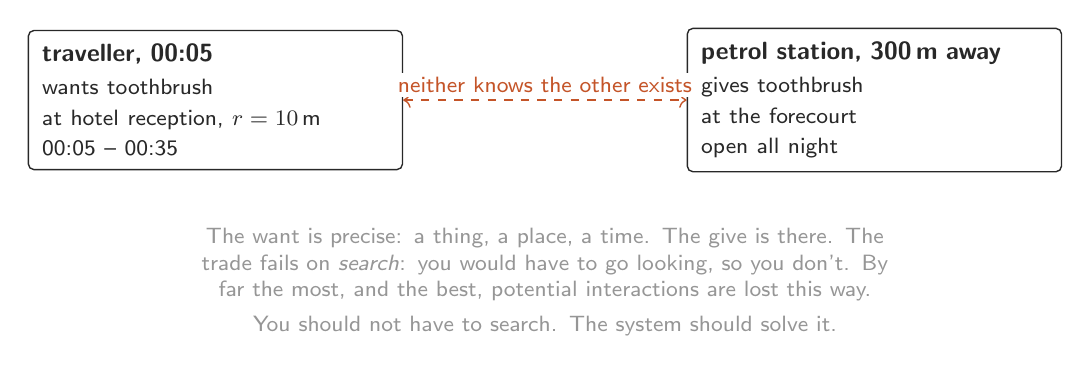
\begin{tikzpicture}
  % The trade that exists and never happens: the want is precise in place
  % and time, the give is 300 m away, and nobody is searching.
  \node[maker, align=left, text width=44mm] (W) {\textbf{traveller, 00:05}\\[1pt]{\footnotesize wants toothbrush}\\{\footnotesize at hotel reception, $r = 10$\,m}\\{\footnotesize 00:05 -- 00:35}};
  \node[maker, align=left, text width=44mm, right=36mm of W] (G) {\textbf{petrol station, 300\,m away}\\[1pt]{\footnotesize gives toothbrush}\\{\footnotesize at the forecourt}\\{\footnotesize open all night}};
  \draw[wrong, dashed, <->] (W) -- node[lbl, text=warn, above=1pt] {neither knows the other exists} (G);
  \node[note, anchor=north, text width=110mm] at ($(W.south)!0.5!(G.south) + (0,-6mm)$) {The want is precise: a thing, a place, a time. The give is there. The trade fails on \emph{search}: you would have to go looking, so you don't. By far the most, and the best, potential interactions are lost this way.\\[3pt] You should not have to search. The system should solve it.};
\end{tikzpicture}
\end{document}
